% Rozwinięcie AM II-03 i AM II-04; dyskretne odpowiedniki twierdzeń z TM-12.
\chapter{Rodziny sumowalne i szeregi wielokrotne}
\label{ma2:ch:summable-families}

W rozdziale \ref{ma2:ch:unconditional-series} badaliśmy
sumy po skończonych zbiorach indeksów szeregu. Teraz
zbiór indeksów nie musi być przeliczalny ani uporządkowany.
Rozwiniemy teorię bez odwoływania się do całki Lebesgue'a.
W przypadku przeliczalnych zbiorów indeksów otrzymamy
dyskretne odpowiedniki twierdzeń Tonellego i Fubiniego
(teoria miary, rozdział 12, etykiety
\texttt{thm:tonelli-12} i \texttt{thm:fubini-12}).
Dowody ogólnych twierdzeń miarowych pozostają w tamtym skrypcie.

\section{Sumy rodzin nieujemnych}

\begin{definicja}
\label{ma2:def:positive-family}
Dla dowolnego zbioru $I$ oraz rodziny
$(a_i)_{i\in I}$ o wartościach w $[0,+\infty]$ określamy
\[
 \sum_{i\in I}a_i
 :=\sup\left\{\sum_{i\in F}a_i:
                 F\subseteq I,\ F\text{ skończony}\right\}.
\]
Suma pusta wynosi $0$. Jeżeli skończona suma zawiera
składnik $+\infty$, przyjmuje wartość $+\infty$.
\end{definicja}
Jeżeli $I=\N_+$, definicja zgadza się z granicą
niemalejących sum częściowych. Istotnie, każdy skończony
zbiór indeksów jest zawarty w pewnym początkowym
przedziale, a każdy taki przedział jest dopuszczalny
w supremum. Jest to rozszerzenie definicji z AM I,
rozdział 09, sekcja o szeregach nieujemnych.

\begin{lemat}[Monotoniczność i skończony podział]
\label{ma2:lem:positive-family-partition}
Jeżeli $a_i\le b_i$ dla wszystkich $i\in I$, to
$\sum_{i\in I}a_i\le\sum_{i\in I}b_i$.
Jeżeli $I=A\cup B$, $A\cap B=\varnothing$, to
\[
 \sum_{i\in I}a_i=\sum_{i\in A}a_i+\sum_{i\in B}a_i.
\]
\end{lemat}
\begin{proof}
Pierwsza teza wynika z porównania każdej skończonej sumy.
Dla drugiej oznaczmy sumy po $A,B$ przez $\alpha,\beta$.
Rozkładając każdy skończony $F\subseteq I$ na rozłączne
części $F\cap A$ i $F\cap B$, otrzymujemy
$\sum_{i\in F}a_i\le\alpha+\beta$. Bierzemy supremum po $F$.
Jeżeli $\alpha,\beta$ są skończone, to dla każdego
$\varepsilon>0$ wybieramy skończone $F_A\subseteq A$,
$F_B\subseteq B$ o sumach większych niż
$\alpha-\varepsilon/2$ i $\beta-\varepsilon/2$.
Ich suma zbiorów jest skończona i rozłączna, więc
$\sum_{i\in I}a_i>\alpha+\beta-\varepsilon$.
Dowolność $\varepsilon$ daje nierówność odwrotną.
Jeżeli któraś z liczb $\alpha,\beta$ jest nieskończona,
to sumy po odpowiednich skończonych podzbiorach
są dowolnie duże (lub nieskończone), a zatem
$\sum_{i\in I}a_i=+\infty$.
\end{proof}

\begin{twierdzenie}[Przeliczalność nośnika i oszacowanie ogona]
\label{ma2:thm:positive-family-support}
Jeżeli $\alpha=\sum_{i\in I}a_i<\infty$, to zbiór
$\{i\in I:a_i>0\}$ jest co najwyżej przeliczalny.
Ponadto dla każdego $\varepsilon>0$ istnieje skończony
$F_0\subseteq I$ taki, że
$\sum_{i\in I\setminus F_0}a_i<\varepsilon$.
\end{twierdzenie}
\begin{proof}
Dla $m\ge1$ zbiór $A_m=\{i:a_i\ge1/m\}$ jest skończony:
gdyby zawierał $r$ różnych elementów przy $r>m\alpha$,
suma po nich byłaby co najmniej $r/m>\alpha$.
Każde dodatnie $a_i$ należy do jednego z tych progów,
więc $\{i:a_i>0\}=\bigcup_{m\ge1}A_m$.
Jest to przeliczalna suma zbiorów skończonych, a więc
zbiór co najwyżej przeliczalny.
Z definicji supremum wybieramy skończony $F_0$
z $\sum_{i\in F_0}a_i>\alpha-\varepsilon$.
Lemat \ref{ma2:lem:positive-family-partition} daje
$\sum_{i\in I\setminus F_0}a_i
=\alpha-\sum_{i\in F_0}a_i<\varepsilon$.
\end{proof}

\section{Rodziny w przestrzeniach unormowanych}

\begin{definicja}
\label{ma2:def:summable-family}
Niech $E$ będzie przestrzenią unormowaną nad $\K$,
$I$ dowolnym zbiorem, a $(x_i)_{i\in I}$ rodziną w $E$.
Dla skończonego $F\subseteq I$ piszemy
$S_F=\sum_{i\in F}x_i$. Rodzinę nazywamy sumowalną
do $S\in E$, gdy dla każdego $\varepsilon>0$ istnieje
skończony $F_0\subseteq I$ taki, że
$\|S_F-S\|<\varepsilon$ dla każdego skończonego
$F\supseteq F_0$. Piszemy wówczas $\sum_{i\in I}x_i=S$.
Jest to zbieżność sieci sum skończonych skierowanej
przez inkluzję: dla dwóch skończonych zbiorów ich suma
jest wspólnym większym elementem.
Rodzinę nazywamy bezwzględnie sumowalną, gdy
$\sum_{i\in I}\|x_i\|<\infty$.
\end{definicja}
Suma rodziny, jeśli istnieje, jest jednoznaczna.
Jeżeli $S,T$ spełniają definicję, to dla $\varepsilon>0$
bierzemy sumę dwóch zbiorów progowych z dokładnością
$\varepsilon/2$. Dla tego zbioru $F$ zachodzi
$\|S-T\|\le\|S-S_F\|+\|S_F-T\|<\varepsilon$, więc $S=T$.
Przypadek pustego $I$ daje sumę $0$.
Z definicji wynika liniowość sumowania: dla dwóch
sumowalnych rodzin na tym samym zbiorze indeksów
i skalarów $\alpha,\beta$ wybieramy wspólny próg
dla dokładności $\varepsilon/(1+|\alpha|+|\beta|)$.
Nierówność trójkąta dla skończonych sum daje
$\sum_i(\alpha x_i+\beta y_i)=\alpha\sum_i x_i+\beta\sum_i y_i$.

\begin{twierdzenie}[Kryterium Cauchy'ego dla rodzin]
\label{ma2:thm:family-cauchy}
Jeżeli $(x_i)_{i\in I}$ jest sumowalna, to
\begin{equation}
\label{ma2:eq:family-tail}
 \forall\varepsilon>0\ \exists F_0\subseteq I
 \text{ skończony}\quad
 \left\|\sum_{i\in H}x_i\right\|<\varepsilon
\end{equation}
dla każdego skończonego $H\subseteq I\setminus F_0$.
Jeżeli $E$ jest przestrzenią Banacha, warunek ten
jest również wystarczający.
\end{twierdzenie}
\begin{proof}
Dla rodziny sumowalnej do $S$ wybieramy próg $F_0$
dla dokładności $\varepsilon/2$. Dla $H$ jak w tezie
mamy $S_H=S_{F_0\cup H}-S_{F_0}$, zatem
$\|S_H\|<\varepsilon$.

Odwrotnie, dla każdego $n\ge1$ wybieramy skończony
$D_n\subseteq I$ spełniający warunek dla $2^{-n}$.
Niech $F_n=\bigcup_{j=1}^nD_j$. Zbiory $F_n$ są
skończone i rosnące. Dla $m\ge n$ zbiór
$F_m\setminus F_n$ jest rozłączny z $D_n$, więc
$\|S_{F_m}-S_{F_n}\|<2^{-n}$. Ciąg $(S_{F_n})$
jest ciągiem Cauchy'ego, zatem w przestrzeni Banacha
ma granicę $S$. Przechodząc do granicy po $m$ w
nierówności, dostajemy $\|S-S_{F_n}\|\le2^{-n}$.
Jeśli $F\supseteq F_n$ jest skończony, to również
$\|S_F-S_{F_n}\|<2^{-n}$, gdyż $F\setminus F_n$
nie przecina $D_n$. Stąd $\|S_F-S\|<2^{1-n}$.
Dla każdego $\varepsilon>0$ wybór $n$ z $2^{1-n}<\varepsilon$
daje zbieżność całej sieci, nie tylko wybranego ciągu.
\end{proof}

\begin{wniosek}
\label{ma2:cor:family-support}
Rodzina spełniająca warunek \eqref{ma2:eq:family-tail}
ma co najwyżej przeliczalny nośnik
$J=\{i\in I:x_i\ne0\}$.
Jeżeli rodzina jest sumowalna, to jej suma jest równa
sumie ograniczenia do $J$.
\end{wniosek}
\begin{proof}
Dla $m\ge1$ wybieramy $F_m$ dla $\varepsilon=1/m$.
Stosując warunek do singletonu poza $F_m$, widzimy,
że $\{i:\|x_i\|\ge1/m\}\subseteq F_m$. Zatem $J$
jest przeliczalną sumą zbiorów skończonych.
Jeżeli $F_0$ jest progiem sumowalności w $I$, to
$F_0\cap J$ jest progiem w $J$: dla skończonego
$G\subseteq J$ zawierającego $F_0\cap J$ mamy
$S_G=S_{G\cup F_0}$, gdyż dodane indeksy mają
wyrazy zerowe. Odwrotnie, próg w $J$ działa także
w $I$, ponieważ $S_F=S_{F\cap J}$.
\end{proof}

\begin{twierdzenie}[Związek z szeregami]
\label{ma2:thm:family-enumeration}
Niech $E$ będzie przestrzenią Banacha, a $J$
nieskończonym przeliczalnym nośnikiem rodziny.
Dla dowolnej bijekcji $\pi:\N_+\to J$ rodzina jest
sumowalna wtedy i tylko wtedy, gdy szereg
$\sum_{n\ge1}x_{\pi(n)}$ jest bezwarunkowo zbieżny.
Wtedy obie sumy są równe i nie zależą od $\pi$.
Dla skończonego nośnika suma jest zwykłą sumą skończoną.
\end{twierdzenie}
\begin{proof}
Z wniosku \ref{ma2:cor:family-support} wystarczy
rozpatrzyć rodzinę na $J$ (również gdy sumowalność
ograniczenia jest założeniem). Bijekcja $\pi$
przenosi skończone podzbiory $\N_+$ na wszystkie
skończone podzbiory $J$, zachowując inkluzję.
Warunek z definicji \ref{ma2:def:summable-family}
jest więc dokładnie warunkiem zbieżności sieci sum
skończonych szeregu. Równoważność i równość sum
wynikają z twierdzenia \ref{ma2:thm:unconditional-finite}.
Dla skończonego nośnika można obrać cały $J$ jako
zbiór progowy dla dowolnej dokładności.
\end{proof}

\begin{twierdzenie}[Sumowalność bezwzględna]
\label{ma2:thm:absolute-family}
W przestrzeni Banacha każda rodzina bezwzględnie
sumowalna jest sumowalna. Jeżeli $S$ jest jej sumą,
to dla każdego skończonego $F\subseteq I$
\[
 \|S-S_F\|\le\sum_{i\in I\setminus F}\|x_i\|.
\]
\end{twierdzenie}
\begin{proof}
Twierdzenie \ref{ma2:thm:positive-family-support}
zastosowane do $a_i=\|x_i\|$ daje dla każdego
$\varepsilon>0$ skończony $F_0$ z sumą norm poza
nim mniejszą od $\varepsilon$. Nierówność trójkąta
daje warunek \eqref{ma2:eq:family-tail}, więc
twierdzenie \ref{ma2:thm:family-cauchy} zapewnia
istnienie $S$. Dla dowolnego $\delta>0$ wybieramy
skończony $G$ zawierający $F$ i próg sumowalności
dla $\delta$. Wówczas
\[
 \|S-S_F\|\le\|S-S_G\|+\|S_{G\setminus F}\|
 <\delta+\sum_{i\in I\setminus F}\|x_i\|.
\]
Dowolność $\delta$ kończy dowód.
\end{proof}

\begin{uwaga}
Zbieżność bezwarunkowa nie musi oznaczać sumowalności
bezwzględnej w nieskończenie wymiarowej przestrzeni
Banacha: przykład \ref{ma2:ex:unconditional-l2}
daje rodzinę $(e_n/n)$ w $\ell^2$.
W skończonym wymiarze obie własności są równoważne,
na mocy wniosku \ref{ma2:cor:family-support},
twierdzenia \ref{ma2:thm:family-enumeration} i twierdzenia
\ref{ma2:thm:finite-unconditional-absolute}.
\end{uwaga}

\section{Sumowanie po rozłącznych częściach}

\begin{twierdzenie}[Dyskretne twierdzenie Tonellego]
\label{ma2:thm:family-tonelli}
Niech $I=\bigcup_{j\in J}I_j$, gdzie $(I_j)_{j\in J}$
jest rodziną parami rozłącznych zbiorów; dopuszczamy
zbiory puste. Dla $a_i\in[0,+\infty]$ zachodzi
\[
 \sum_{i\in I}a_i=\sum_{j\in J}\sum_{i\in I_j}a_i
\]
w $[0,+\infty]$.
\end{twierdzenie}
\begin{proof}
Oznaczmy lewą stronę przez $A$, a wewnętrzne sumy
przez $b_j$. Każdy skończony $F\subseteq I$
przecina tylko skończenie wiele części $I_j$;
oznaczmy ich indeksy przez $J_F$.
Z rozłączności mamy
$\sum_{i\in F}a_i=\sum_{j\in J_F}\sum_{i\in F\cap I_j}a_i
\le\sum_{j\in J}b_j$. Biorąc supremum po $F$,
otrzymujemy pierwszą nierówność.
Jeżeli $A=+\infty$, równość już wynika.
Niech więc $A<\infty$. Z monotoniczności
$b_j\le A$ dla każdego $j$. Dla dowolnego niepustego
skończonego $K\subseteq J$ i $\varepsilon>0$ wybieramy
skończone $F_j\subseteq I_j$ z
$\sum_{i\in F_j}a_i>b_j-\varepsilon/|K|$.
Suma zbiorów $F_j$ dla $j\in K$ jest skończona
i rozłączna, więc
$\sum_{j\in K}b_j<A+\varepsilon$.
Dowolność $\varepsilon$ daje $\sum_{j\in K}b_j\le A$;
dla pustego $K$ nierówność również zachodzi.
Biorąc supremum po $K$, otrzymujemy tezę.
\end{proof}

\begin{twierdzenie}[Grupowanie rodziny sumowalnej]
\label{ma2:thm:family-grouping}
Niech $E$ będzie przestrzenią Banacha, $(x_i)_{i\in I}$
rodziną sumowalną do $S$, a $(I_j)_{j\in J}$
podziałem $I$ na parami rozłączne części, z dopuszczeniem
części pustych. Każde ograniczenie do $I_j$ jest
sumowalne, a rodzina $y_j=\sum_{i\in I_j}x_i$
jest sumowalna i $\sum_{j\in J}y_j=S$.
Jeżeli rodzina wyjściowa jest bezwzględnie sumowalna,
to
\[
 \sum_{j\in J}\|y_j\|\le\sum_{i\in I}\|x_i\|.
\]
\end{twierdzenie}
\begin{proof}
Warunek \eqref{ma2:eq:family-tail} dla dowolnego
podzbioru $B\subseteq I$ wynika z warunku dla $I$:
wystarczy przeciąć zbiór progowy z $B$. Twierdzenie
\ref{ma2:thm:family-cauchy} daje sumowalność
każdego ograniczenia. Dla skończonego $K\subseteq J$
niech $B_K=\bigcup_{j\in K}I_j$.
Wykażemy $\sum_{i\in B_K}x_i=\sum_{j\in K}y_j$.
Dla $K=\varnothing$ jest to równość zer.
Dla $K\ne\varnothing$ i $\varepsilon>0$ wybieramy
w każdej części próg $D_j\subseteq I_j$ dla
dokładności $\varepsilon/|K|$. Dla dowolnego
skończonego $F\subseteq B_K$ zawierającego
$\bigcup_{j\in K}D_j$ zachodzi
\[
 \left\|\sum_{i\in F}x_i-\sum_{j\in K}y_j\right\|
 \le \sum_{j\in K}\left\|\sum_{i\in F\cap I_j}x_i-y_j\right\|
 <\varepsilon.
\]
Jednoznaczność sumy daje żądaną równość.

Ustalmy $\varepsilon>0$ i wybierzmy skończony $F_0$
z definicji sumowalności $S$ dla dokładności
$\varepsilon/2$. Niech $K_0$ będzie skończonym zbiorem
indeksów części przecinających $F_0$. Dla każdego
skończonego $K\supseteq K_0$ mamy $F_0\subseteq B_K$.
Niech $F\subseteq B_K$ będzie skończony, zawiera $F_0$
oraz próg sumowalności ograniczenia do $B_K$ dla
$\varepsilon/2$. Wtedy
\[
 \left\|\sum_{j\in K}y_j-S\right\|
 \le \left\|\sum_{i\in B_K}x_i-S_F\right\|+\|S_F-S\|
 <\varepsilon.
\]
To dowodzi sumowalności rodziny $(y_j)$ do $S$.
Jeżeli ponadto suma norm rodziny wyjściowej jest
skończona, z twierdzenia \ref{ma2:thm:absolute-family}
dla $F=\varnothing$ mamy
$\|y_j\|\le\sum_{i\in I_j}\|x_i\|$.
Monotoniczność i twierdzenie \ref{ma2:thm:family-tonelli}
dają ostatnią nierówność.
\end{proof}

\section{Szeregi podwójne i wielokrotne}

\begin{wniosek}[Dyskretne twierdzenia Tonellego i Fubiniego]
\label{ma2:cor:double-fubini}
Niech $I,J$ będą dowolnymi zbiorami.
Dla $a_{ij}\in[0,+\infty]$ zachodzi
\[
 \sum_{(i,j)\in I\times J}a_{ij}
 =\sum_{i\in I}\sum_{j\in J}a_{ij}
 =\sum_{j\in J}\sum_{i\in I}a_{ij}.
\]
Dla rodziny sumowalnej $(x_{ij})$ w przestrzeni
Banacha zachodzą te same równości w tej przestrzeni,
a każda z wewnętrznych i zewnętrznych rodzin
jest sumowalna. W szczególności wystarcza
$\sum_{(i,j)\in I\times J}\|x_{ij}\|<\infty$.
\end{wniosek}
\begin{proof}
Stosujemy twierdzenie \ref{ma2:thm:family-tonelli}
lub \ref{ma2:thm:family-grouping} do dwóch podziałów
$I\times J$: na części $\{i\}\times J$ oraz na części
$I\times\{j\}$. W przypadku sumy norm istnienie
sumy zapewnia twierdzenie \ref{ma2:thm:absolute-family}.
Każda z części jest w naturalnej bijekcji z odpowiednim
zbiorem indeksów, co nie zmienia skończonych sum.
\end{proof}

Dla $I=J=\N_+$ możemy używać klasycznej notacji
szeregów iterowanych. Jeżeli rodzina jest sumowalna
do $S$, jej sumy prostokątne
\[
 R_{mn}=\sum_{i=1}^m\sum_{j=1}^n x_{ij}
\]
dążą do $S$ w sensie Pringsheima: dla każdego
$\varepsilon>0$ istnieje $N$, że
$\|R_{mn}-S\|<\varepsilon$ dla $m,n\ge N$.
Istotnie, każdy skończony zbiór progowy jest zawarty
w pewnym kwadracie $\{1,\ldots,N\}^2$.
Zależności między tymi sposobami sumowania nie są
odwracalne bez dodatkowych założeń.

\begin{przyklad}[Różne sumy iterowane]
\label{ma2:ex:double-different}
Dla $i,j\ge1$ połóżmy $a_{ij}=1$ przy $j=i$,
$a_{ij}=-1$ przy $j=i+1$ i $a_{ij}=0$ w pozostałych
przypadkach. Każdy wiersz ma dwa niezerowe wyrazy,
których suma wynosi $0$. Pierwsza kolumna ma jeden
niezerowy wyraz $1$, a każda następna ma dwa
wyrazy $1,-1$. Zatem
\[
 \sum_{i=1}^{\infty}\sum_{j=1}^{\infty}a_{ij}=0,
 \qquad
 \sum_{j=1}^{\infty}\sum_{i=1}^{\infty}a_{ij}=1.
\]
Rodzina nie jest bezwzględnie sumowalna, ponieważ
suma modułów po $N$ punktach przekątnej wynosi $N$.
Nie jest też sumowalna z wniosku
\ref{ma2:cor:double-fubini}.
Sumy prostokątne są równe $1$ dla $n\le m$ i $0$
dla $n>m$: liczba dodatnich składników to
$\min(m,n)$, a ujemnych $\min(m,n-1)$.
Sumy kwadratowe są więc stałe, ale granica w sensie
Pringsheima nie istnieje.
\end{przyklad}

\begin{figure}[htbp]
\centering
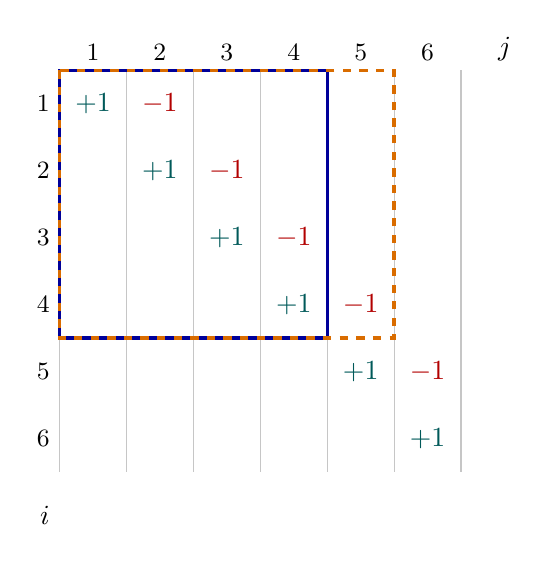
\begin{tikzpicture}[x=.85cm,y=-.85cm]
\draw[step=1,gray!45] (0,0) grid (6,6);
\foreach \i in {1,...,6}{
 \node[above] at (\i-.5,0) {\small \i};
 \node[left] at (0,\i-.5) {\small \i};
 \node[teal!70!black] at (\i-.5,\i-.5) {$+1$};
}
\foreach \i in {1,...,5}{
 \node[red!70!black] at (\i+.5,\i-.5) {$-1$};
}
\node[above] at (6.65,0) {$j$};
\node[left] at (0,6.65) {$i$};
\draw[very thick,blue!60!black] (0,0) rectangle (4,4);
\draw[very thick,orange!85!black,dashed] (0,0) rectangle (5,4);
\end{tikzpicture}
\caption{Rodzina z przykładu \ref{ma2:ex:double-different}.
Niewypełnione pola oznaczają zera. Niebieski kwadrat
ma sumę $1$, a pomarańczowy prostokąt ma sumę $0$.}
\label{ma2:fig:double-different}
\end{figure}
\FloatBarrier

\begin{przyklad}[Granica prostokątna bez sum wierszy]
\label{ma2:ex:rectangular-not-iterated}
Niech $a_{1j}=(-1)^j$, $a_{2j}=-(-1)^j$,
a $a_{ij}=0$ dla $i\ge3$. Dla wszystkich $m\ge2$
i $n\ge1$ mamy $R_{mn}=0$, więc granica prostokątna
istnieje i jest równa $0$. Jednak sumy częściowe
pierwszego wiersza przyjmują naprzemiennie wartości
$-1,0$, a drugiego $1,0$. Żaden z tych szeregów
nie jest zbieżny. Zatem istnienie granicy prostokątnej
nie wystarcza nawet do określenia sumy iterowanej
po wierszach.
\end{przyklad}

\begin{wniosek}[Więcej niż dwa indeksy]
\label{ma2:cor:multiple-family}
Niech $r\ge1$ i $I_1,\ldots,I_r$ będą dowolnymi
zbiorami. Dla nieujemnej rodziny na $I_1\times\cdots\times I_r$
lub rodziny sumowalnej w przestrzeni Banacha
suma całej rodziny jest równa każdej z $r!$
sum iterowanych, z dowolną kolejnością indeksów.
W przypadku nieujemnym dopuszczamy wartość $+\infty$.
\end{wniosek}
\begin{proof}
Dla $r=1$ teza jest definicją. Załóżmy tezę dla $r-1$
i wybierzmy dowolny pierwszy indeks zewnętrzny.
Podzielmy iloczyn kartezjański na włókna dla
ustalonej wartości tego indeksu. Twierdzenie
\ref{ma2:thm:family-tonelli} lub
\ref{ma2:thm:family-grouping} daje sumowalność
odpowiednich rodzin wewnętrznych (w przypadku
nieujemnym są określone przez supremum) oraz
równość sumy z sumą po wybranym indeksie zewnętrznym.
Do każdego włókna stosujemy założenie indukcyjne
dla wybranej kolejności pozostałych $r-1$ indeksów.
Ponieważ wybór kolejności był dowolny, indukcja
kończy dowód.
\end{proof}

\section{Zastosowanie do iloczynów szeregów}

Jeśli $T:E\times F\to G$ jest ciągłym odwzorowaniem
dwuliniowym, $E,F,G$ są przestrzeniami Banacha
oraz $\sum_i\|x_i\|=\alpha<\infty$,
$\sum_j\|y_j\|=\beta<\infty$, to dla stałej $K$
z lematu \ref{ma2:lem:bilinear-bound} mamy
\[
 \sum_{(i,j)\in I\times J}\|T(x_i,y_j)\|
 \le K\alpha\beta.
\]
Istotnie, dla każdego skończonego zbioru par jego
rzuty na $I,J$ są skończone, a rozszerzenie sumy norm
na iloczyn tych rzutów daje oszacowanie przez
$K\alpha\beta$. Bierzemy supremum.
Twierdzenie \ref{ma2:thm:absolute-family} daje
sumowalność rodziny. Dla ustalonego $i$ ciągłe
odwzorowanie liniowe $v\mapsto T(x_i,v)$ zachowuje
granice sieci sum skończonych: z oszacowania
dwuliniowego norma różnicy jest nie większa niż
$K\|x_i\|$ razy norma różnicy odpowiedniej sumy
skończonej i jej granicy. Analogicznie dla drugiego
argumentu. Z wniosku \ref{ma2:cor:double-fubini}
otrzymujemy
\[
 \sum_{(i,j)\in I\times J}T(x_i,y_j)
 =T\left(\sum_{i\in I}x_i,\sum_{j\in J}y_j\right).
\]
Dla przeliczalnych rodzin jest to zgodne z wnioskiem
\ref{ma2:cor:bilinear-pair-enumeration} z rozdziału
o iloczynach Cauchy'ego, który nie wymagał zupełności
przestrzeni przy istniejących sumach.

W kolejnym rozdziale przejdziemy do algebr Banacha
i szeregu Neumanna.
